\chapter{Неопределённость, теорема Эренфеста и классический предел}

\section{Нерешённый вопрос о линейном гамильтониане}

Модель
\begin{equation}
H=cP
\label{eq:l10-linear-hamiltonian}
\end{equation}
была полезна потому, что её волновые пакеты сдвигаются без изменения формы. Однако она содержит и серьёзное предостережение. Импульс может быть положительным или отрицательным, поэтому одна и та же формула приписывает одной плоской волне положительную энергию, а другой — отрицательную:
\begin{equation}
\psi_p(x)=e^{ipx/\hbar},
\qquad
E(p)=cp.
\end{equation}
Если бы сколь угодно много физических частиц могли занимать состояния с отрицательной энергией, пустое пространство не было бы состоянием наименьшей энергии. Оно могло бы порождать кванты с положительной энергией, помещая компенсирующую отрицательную энергию в новые частицы, сохраняя полную энергию, но неограниченно понижая энергию вакуума.

\begin{classroomqa}
\audiencequestion{Почему ветвь с отрицательной энергией — это не просто странный выбор нуля энергии?}
\lecturerresponse{Одинаковый аддитивный сдвиг всех энергий безвреден. Неограниченный снизу спектр — другое дело. Если можно заселять состояния со всё меньшей энергией, а частицы с положительной энергией уносят соответствующий баланс, устойчивого основного состояния нет. Для устойчивости нужна нижняя граница относительно вакуума.}
\end{classroomqa}

\begin{figure}[htbp]
\centering
\includegraphics[width=0.88\textwidth]{lecture_10_figure_01.png}
\caption{Линейный гамильтониан и его собственные функции в виде плоских волн выявляют ветвь отрицательной энергии при \(p<0\).}
\lectureframe{00:04:35}
\end{figure}

Исторический ответ Дирака работал для фермионов. Фермионы подчиняются принципу запрета: никакие два тождественных фермиона не могут находиться в одном и том же одночастичном состоянии. Представим, что заполнены все состояния с отрицательной энергией. Когда все они заняты, принцип запрета не позволяет ещё одному фермиону упасть в этот сектор. Дырка в заполненном множестве ведёт себя как античастица.

Этот аргумент не спасает бозоны с отрицательной энергией. Сколь угодно много бозонов могут занимать одно состояние, поэтому бозонную моду с отрицательной энергией можно было бы заселять без ограничения. Старую картину заполненного моря лучше рассматривать как исторический путь к античастицам; современная квантовая теория поля организует частицы и античастицы, не трактуя физический вакуум как буквальное море наблюдаемых электронов с отрицательной энергией. Здесь нужен более узкий вывод: игрушечный гамильтониан не является полной устойчивой теорией частиц.

Как одномерная карикатура фермионной частицы, движущейся с фиксированной скоростью, эта модель намекает на проблему нейтрино, для которой идеи Дирака были релевантны. Она не может служить теорией фотонов: фотоны — бозоны, и принцип запрета не может заполнить и заблокировать их состояния с отрицательной энергией.

\begin{classroomqa}
\audiencequestion{Почему принцип запрета может стабилизировать фермионную конструкцию, но не бозонную?}
\lecturerresponse{Фермионное состояние можно заполнить один раз, после чего оно блокируется. У бозонного состояния такого предела заполнения нет, поэтому бозонная мода с отрицательной энергией всё равно позволяла бы энергии неограниченно падать.}
\end{classroomqa}

\paragraph{Текущее состояние курса.}
За этот квартал курс охватил значительную часть основ квантовой механики и несколько намеренно простых систем, но очень мало приложений. В частности, он ещё не дошёл даже до гармонического осциллятора. Это упущение обозначает скорее границу, чем завершение: дальше идут теория относительности и теория поля, после чего к квантовой механике нужно будет вернуться, чтобы изучить осциллятор и другие построенные на нём структуры. Устойчивый интерес к более раннему обсуждению запутанности также показывает, почему путь через основы был оправдан.

С этой точки зрения нерешённый вопрос снят. Главный предмет — волновая функция, неопределённость и связь между квантовой эволюцией и классической механикой. Цель состоит не в том, чтобы получить максимально общее возможное уравнение эволюции, а в том, чтобы получить специальное уравнение в координатном представлении, впервые записанное Schr\"odinger.

\section{Волновые функции и полный набор коммутирующих координат}

Для одной частицы на прямой волновая функция в координатном представлении имеет вид
\begin{equation}
\psi(x)=\braket{x}{\psi},
\end{equation}
это амплитуда обнаружить частицу вблизи \(x\). Волновая функция в импульсном представлении имеет вид
\begin{equation}
\widetilde{\psi}(p)=\braket{p}{\psi}.
\end{equation}
Они описывают одно и то же абстрактное состояние в разных базисах и связаны преобразованием Фурье:
\begin{align}
\psi(x)
&=
\int_{-\infty}^{\infty}
\frac{dp}{\sqrt{2\pi\hbar}}\,
\widetilde{\psi}(p)e^{ipx/\hbar},
\label{eq:l10-fourier-forward}\\
\widetilde{\psi}(p)
&=
\int_{-\infty}^{\infty}
\frac{dx}{\sqrt{2\pi\hbar}}\,
\psi(x)e^{-ipx/\hbar}.
\label{eq:l10-fourier-inverse}
\end{align}

\begin{figure}[htbp]
\centering
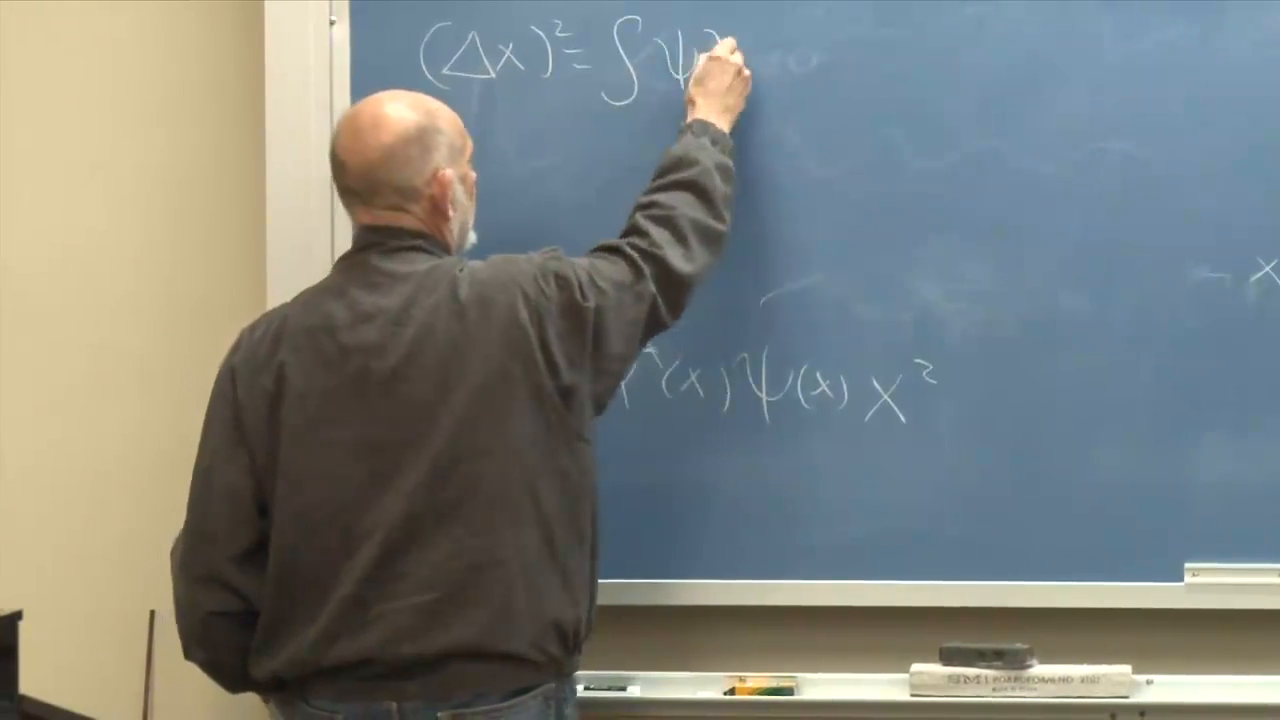
\includegraphics[width=0.88\textwidth]{lecture_10_figure_02.png}
\caption{Координатная и импульсная волновые функции — это проекции одного состояния на два разных непрерывных базиса.}
\lectureframe{00:09:05}
\end{figure}

В двух пространственных измерениях операторы \(X\) и \(Y\) коммутируют, поэтому общий собственный базис можно пометить обеими координатами, и волновая функция принимает вид \(\psi(x,y)\). Эта коммутативность не вынуждается одними лишь абстрактными аксиомами; она является частью эмпирически успешного квантового описания обычного пространства. Для \(N\) частиц в трёх измерениях
\begin{equation}
\psi(\mathbf{x}_1,\ldots,\mathbf{x}_N)
\end{equation}
есть функция на конфигурационном пространстве, а не отдельная трёхмерная волна, независимо приписанная каждой частице. Поэтому для макроскопической системы может потребоваться огромное число координат.

\begin{classroomqa}
\audiencequestion{Следует ли коммутативность различных пространственных координат автоматически из квантовой механики?}
\lecturerresponse{Нет. Абстрактный формализм допускает многие алгебры наблюдаемых. То, что различные декартовы компоненты положения коммутируют, — это эмпирический структурный факт о квантовой механике частиц в обычном пространстве.}
\end{classroomqa}

Можно выполнить преобразование Фурье по каждой координате, получив волновую функцию всех импульсов, или преобразовать только выбранные переменные. Смешанные представления допустимы, потому что представление — это выбор базиса, а не изменение физического состояния.

\section{Что измеряет неопределённость}

Самая элементарная форма принципа неопределённости сразу следует из пары Фурье. Состояние с определённым импульсом представляет собой плоскую волну с постоянным модулем и без локализации по положению. Состояние, резко локализованное по положению, требует многих импульсных компонент. В более общем случае сужение одного члена пары Фурье расширяет другой.

\begin{figure}[htbp]
\centering
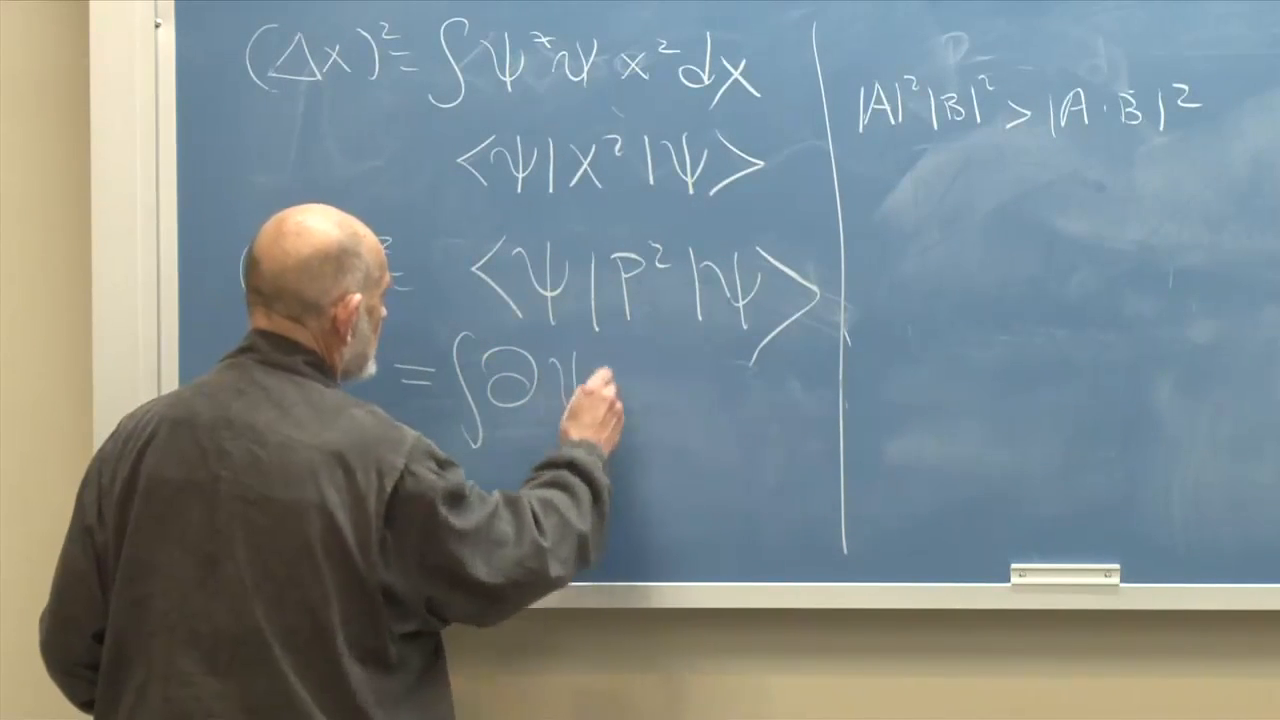
\includegraphics[width=0.88\textwidth]{lecture_10_figure_03.png}
\caption{Локализованный профиль по координате требует широкой суперпозиции плоских волн в сопряжённом импульсном представлении.}
\lectureframe{00:14:45}
\end{figure}

Чтобы придать этому утверждению количественную форму, начнём с произвольной наблюдаемой \(Q\). Её среднее значение в нормированном состоянии равно
\begin{equation}
\expect{Q}=\bra{\psi}Q\ket{\psi}.
\end{equation}
Дисперсия равна
\begin{equation}
(\Delta Q)^2
=
\expect{\bigl(Q-\expect{Q}\bigr)^2}
=
\expect{Q^2}-\expect{Q}^2.
\label{eq:l10-general-variance}
\end{equation}
Неопределённость \(\Delta Q\) — это положительный квадратный корень из этой дисперсии.

Для координаты можно сначала сдвинуть начало координат так, чтобы \(\expect{X}=0\). Тогда
\begin{equation}
(\Delta x)^2
=
\expect{X^2}
=
\int_{-\infty}^{\infty}
dx\,|\psi(x)|^2x^2.
\label{eq:l10-position-variance}
\end{equation}
Положительные и отрицательные вклады взаимно сокращаются в \(\expect{X}\), но складываются в \(\expect{X^2}\). Поэтому более широкое распределение вероятности имеет большую дисперсию.

\begin{figure}[htbp]
\centering
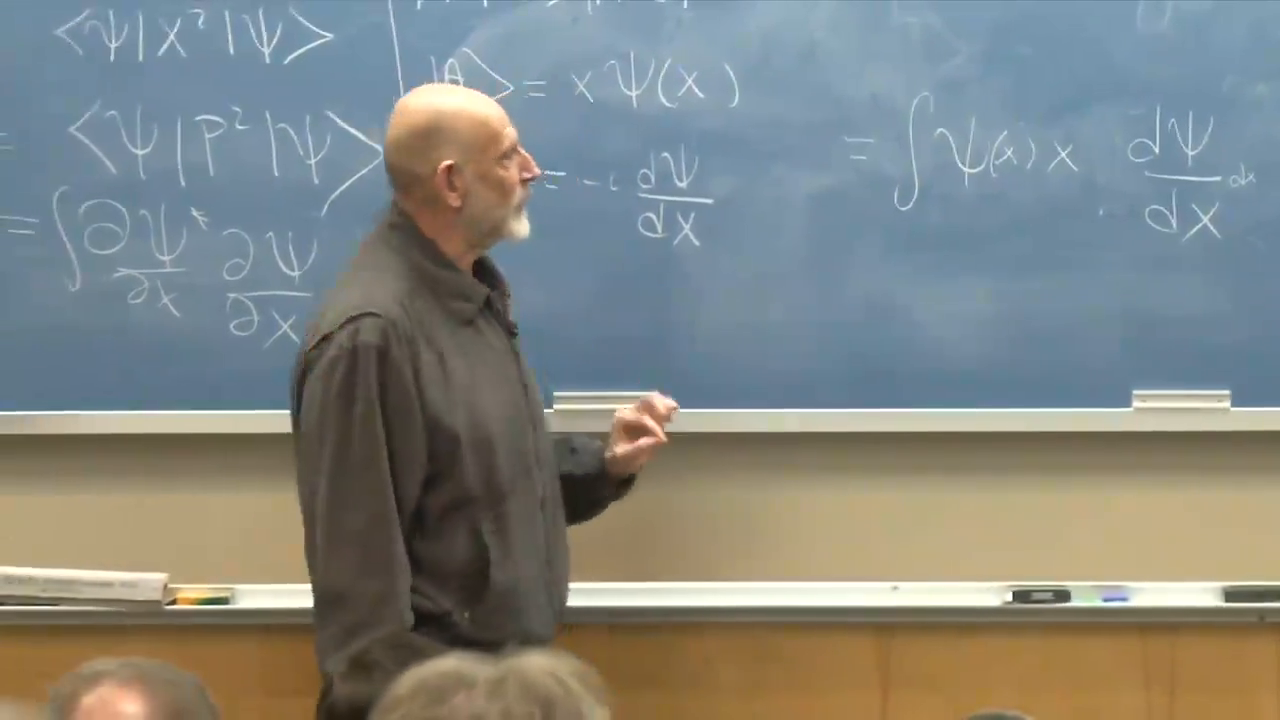
\includegraphics[width=0.88\textwidth]{lecture_10_figure_04.png}
\caption{После сдвига среднего к нулю дисперсия координаты есть интеграл от \(x^2\), взвешенный вероятностью.}
\lectureframe{00:20:50}
\end{figure}

Различие между \(\expect{X^2}\) и \(\expect{X}^2\) существенно. Распределение, симметричное относительно нуля, имеет \(\expect{X}=0\), но, если только оно не сосредоточено в начале координат, всё же имеет \(\expect{X^2}>0\).

Дисперсию импульса можно определить прямо в импульсном пространстве:
\begin{equation}
(\Delta p)^2
=
\int_{-\infty}^{\infty}
dp\,|\widetilde{\psi}(p)|^2
\bigl(p-\expect{P}\bigr)^2.
\end{equation}
Однако для доказательства полезнее работать в координатном пространстве. Сдвинем средний импульс к нулю и воспользуемся
\begin{equation}
P=-i\hbar\frac{d}{dx},
\qquad
P^2=-\hbar^2\frac{d^2}{dx^2}.
\end{equation}
Тогда
\begin{equation}
(\Delta p)^2
=
\expect{P^2}
=
-\hbar^2
\int_{-\infty}^{\infty}
dx\,\psi^*(x)\frac{d^2\psi}{dx^2}.
\label{eq:l10-momentum-variance-second}
\end{equation}

\begin{classroomqa}
\audiencequestion{Как дисперсия может быть положительной, если её формула в координатном пространстве начинается со знака минус?}
\lecturerresponse{Интеграл, стоящий при этом знаке, неположителен. Интегрирование по частям переносит одну производную на \(\psi^*\), вносит второй знак минус и превращает результат в интеграл от квадрата модуля.}
\end{classroomqa}

Для волновых функций, достаточно быстро убывающих на бесконечности,
\begin{equation}
\int f\,g'\,dx
=
\left[fg\right]_{-\infty}^{\infty}
-
\int f'g\,dx,
\end{equation}
и граничный член исчезает. Однократное применение этого к уравнению~\eqref{eq:l10-momentum-variance-second} даёт
\begin{equation}
(\Delta p)^2
=
\hbar^2
\int_{-\infty}^{\infty}
dx\,
\frac{d\psi^*}{dx}
\frac{d\psi}{dx}
=
\hbar^2
\int_{-\infty}^{\infty}
dx\,
\left|\frac{d\psi}{dx}\right|^2
\geq 0.
\label{eq:l10-momentum-variance-positive}
\end{equation}

\begin{figure}[htbp]
\centering
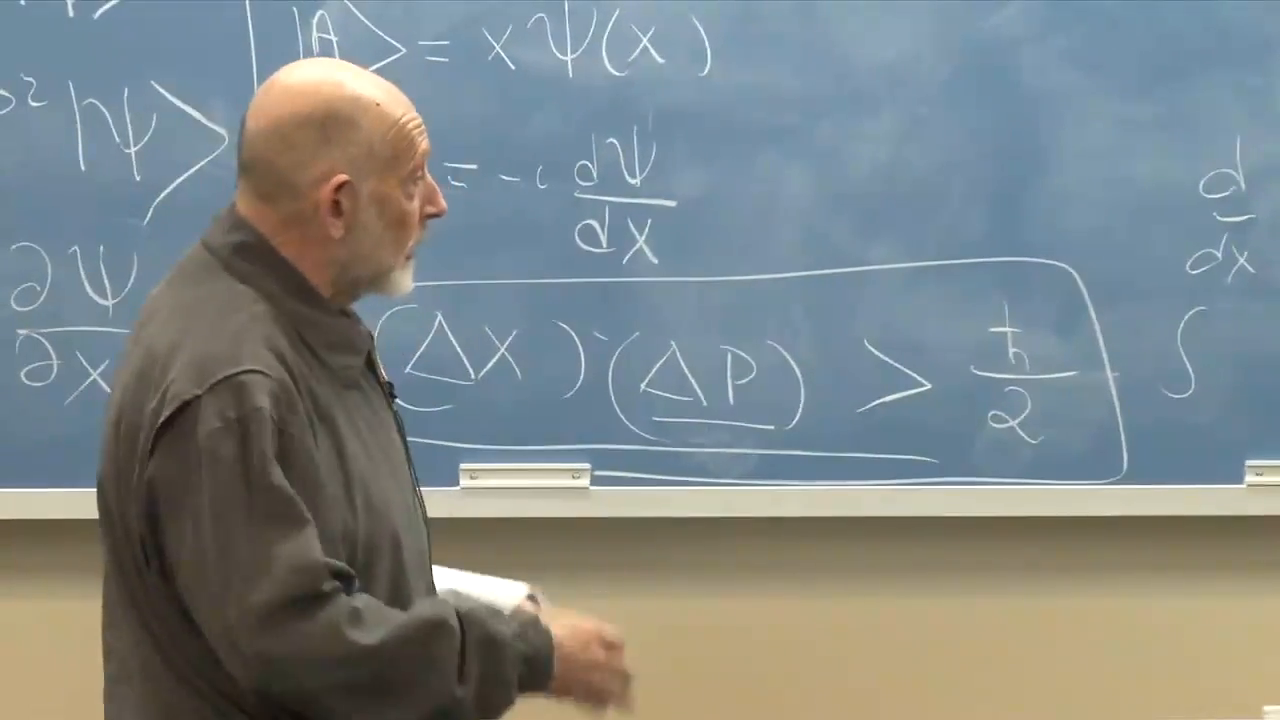
\includegraphics[width=0.88\textwidth]{lecture_10_figure_05.png}
\caption{Интегрирование по частям превращает кажущееся отрицательным выражение для \(\expect{P^2}\) в явно положительную норму.}
\lectureframe{00:27:35}
\end{figure}

\begin{classroomqa}
\audiencequestion{Можно ли одновременно сдвинуть средние значения положения и импульса к нулю?}
\lecturerresponse{Да. Сдвиг аргумента волновой функции изменяет \(\expect{X}\), а умножение её на фазу плоской волны изменяет \(\expect{P}\). Эти операции меняют средние значения, не изменяя соответствующих дисперсий, так что в доказательстве можно использовать обе центрированные величины.}
\end{classroomqa}

\section{Ограничение на неопределённость}

Математический инструмент, который здесь нужен, — это неравенство Коши--Шварца. На лекции к нему подходят через элементарную векторную геометрию: скалярное произведение двух векторов равно произведению их длин на косинус угла между ними, поэтому его модуль не может превышать произведения их длин. В обозначениях пространства Гильберта
\begin{equation}
\braket{A}{A}\braket{B}{B}
\geq
\left|\braket{A}{B}\right|^2.
\label{eq:l10-cauchy-schwarz}
\end{equation}
Оно верно в вещественных и комплексных векторных пространствах любой размерности.

\begin{figure}[htbp]
\centering
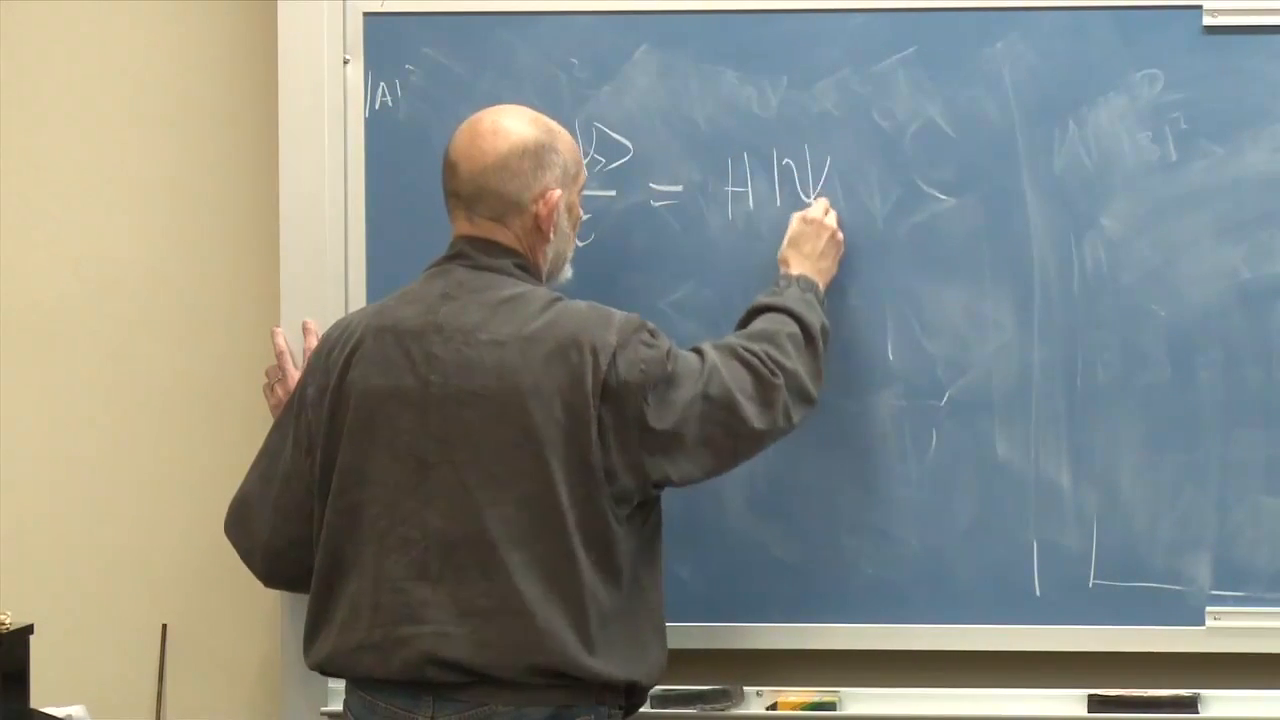
\includegraphics[width=0.88\textwidth]{lecture_10_figure_06.png}
\caption{Геометрическое векторное неравенство переформулируется как оценка Коши--Шварца в пространстве Гильберта, используемая в доказательстве.}
\lectureframe{00:35:35}
\end{figure}

\begin{classroomqa}
\audiencequestion{Должно ли неравенство быть строгим, или возможно равенство?}
\lecturerresponse{Это соотношение типа больше или равно. Равенство имеет место, когда два вектора гильбертова пространства линейно зависимы. Это условие равенства позже выделит волновые пакеты с минимальной неопределённостью.}
\end{classroomqa}

Сместим обе переменные к их средним значениям и сначала проследим упрощённое доказательство у доски, в котором \(\psi(x)\) считается вещественной. Определим
\begin{equation}
\ket{A}=X\ket{\psi},
\qquad
\ket{B}=P\ket{\psi}.
\label{eq:l10-auxiliary-vectors}
\end{equation}
Квадраты их норм в точности равны дисперсиям:
\begin{equation}
\braket{A}{A}=(\Delta x)^2,
\qquad
\braket{B}{B}=(\Delta p)^2.
\end{equation}

\begin{figure}[htbp]
\centering
\includegraphics[width=0.88\textwidth]{lecture_10_figure_07.png}
\caption{Вспомогательные векторы \(X\ket{\psi}\) и \(P\ket{\psi}\) превращают две дисперсии в нормы в гильбертовом пространстве.}
\lectureframe{00:44:40}
\end{figure}

Остаётся скалярное произведение
\begin{align}
\braket{A}{B}
&=
\int_{-\infty}^{\infty}
dx\,
x\psi(x)
\left(-i\hbar\frac{d\psi}{dx}\right).
\end{align}
Входит только его модуль. Поскольку \(\psi\) вещественна,
\begin{equation}
\psi\frac{d\psi}{dx}
=
\frac{1}{2}\frac{d}{dx}\psi^2.
\end{equation}
Следовательно,
\begin{align}
\left|\braket{A}{B}\right|
&=
\frac{\hbar}{2}
\left|
\int_{-\infty}^{\infty}
dx\,
x\frac{d}{dx}\psi^2
\right| \notag\\
&=
\frac{\hbar}{2}
\left|
-\int_{-\infty}^{\infty}
dx\,\psi^2
\right|
=
\frac{\hbar}{2},
\label{eq:l10-inner-product-half-hbar}
\end{align}
где интегрирование по частям снимает производную с \(\psi^2\), \(d x/dx=1\), граничный член обращается в нуль, а нормировка даёт последнее равенство.

Подставим уравнение~\eqref{eq:l10-inner-product-half-hbar} в неравенство Коши--Шварца:
\begin{equation}
(\Delta x)^2(\Delta p)^2
\geq
\frac{\hbar^2}{4}.
\end{equation}
Извлекая положительный квадратный корень, получаем
\begin{equation}
\boxed{
\Delta x\,\Delta p
\geq
\frac{\hbar}{2}
}.
\label{eq:l10-uncertainty-principle}
\end{equation}

\begin{figure}[htbp]
\centering
\includegraphics[width=0.88\textwidth]{lecture_10_figure_08.png}
\caption{Шаг с интегрированием по частям и нормировка дают точную нижнюю границу неопределённости положения и импульса.}
\lectureframe{00:50:55}
\end{figure}

Ограничение на вещественность \(\psi\) было удобством для вывода у доски, а не ограничением самой теоремы. Для общего комплексного состояния возьмём
\begin{equation}
\ket{A}=(X-\expect{X})\ket{\psi},
\qquad
\ket{B}=(P-\expect{P})\ket{\psi}.
\end{equation}
Коммутатор фиксирует мнимую часть их скалярного произведения:
\begin{equation}
\operatorname{Im}\braket{A}{B}
=
\frac{1}{2i}\expect{[X,P]}
=
\frac{\hbar}{2}.
\end{equation}
Поскольку \(|\braket{A}{B}|\) по меньшей мере не меньше модуля его мнимой части, отсюда следует та же самая граница.

\begin{classroomqa}
\audiencequestion{Что именно произошло с граничным членом при повторных интегрированиях по частям?}
\lecturerresponse{Для рассматриваемых здесь нормируемых пакетов произведения, возникающие при \(+\infty\) и \(-\infty\), обращаются в нуль. На конечном периодическом интервале граничные члены на концах сокращаются. Области определения операторов должны быть выбраны так, чтобы эти утверждения выполнялись; иначе формальное преобразование не оправдано.}
\end{classroomqa}

\begin{classroomqa}
\audiencequestion{Знак равенства физически достижим, или нижняя граница — лишь оценка?}
\lecturerresponse{Он достижим. Равенство в неравенстве Коши--Шварца требует, чтобы два вспомогательных вектора были пропорциональны. Решение этого условия даёт гауссовы пакеты, состояния минимальной неопределённости, которые будут рассмотрены далее.}
\end{classroomqa}

\section{Другие фурье-сопряжённые пары}

Соотношение неопределённостей между временем и энергией напоминает соотношение между положением и импульсом. Однако оно требует большей осторожности, потому что время здесь обычно является параметром эволюции, а не наблюдаемой величиной, представленной универсальным самосопряжённым оператором. Разложим состояние по собственным векторам энергии:
\begin{equation}
\ket{\psi(t)}
=
\int dE\,
\phi(E)e^{-iEt/\hbar}\ket{E}.
\label{eq:l10-time-energy-fourier}
\end{equation}
Амплитуды по энергии и временная зависимость связаны преобразованием Фурье. Узкое распределение по энергии меняется медленно и не может образовать резко локализованный по времени импульс; широкое распределение по энергии может дать короткую огибающую времени прихода.

\begin{figure}[htbp]
\centering
\includegraphics[width=0.88\textwidth]{lecture_10_figure_09.png}
\caption{Временная зависимость собирается из собственных состояний энергии с фазами \(e^{-iEt/\hbar}\), образуя фурье-базис для связи между временем и энергией.}
\lectureframe{00:53:40}
\end{figure}

\begin{classroomqa}
\audiencequestion{Применимо ли то же доказательство напрямую к времени и энергии?}
\lecturerresponse{Интуиция взаимной обратности ширин — да, и проходящий волновой пакет даёт полезный пример: короткое окно времени прихода требует широкого распределения по энергии. Операторное утверждение тоньше, потому что время входит в эту формулировку не совсем так, как \(X\).}
\end{classroomqa}

Угол и момент импульса образуют ещё одну сопряжённую пару для вращательного движения. Локально их фурье-связь напоминает связь положения и импульса. Глобально периодичность угла требует дополнительной осторожности, поэтому здесь это замечание служит аналогией, а не полной теоремой.

\begin{classroomqa}
\audiencequestion{Являются ли пары положение-импульс, время-энергия и угол-момент импульса изолированными примерами?}
\lecturerresponse{Нет. Канонически сопряжённые переменные снова и снова возникают как фурье-пары. Детали областей определения и периодичности различаются, но общей структурой служит взаимно-обратная локализация.}
\end{classroomqa}

\section{Уравнение Schr\"odinger в координатном представлении}

Теперь вернёмся к динамике. Абстрактный закон имеет вид
\begin{equation}
i\hbar\frac{d}{dt}\ket{\psi(t)}
=
H\ket{\psi(t)}.
\label{eq:l10-abstract-schrodinger}
\end{equation}
Для частицы массы \(m\) в потенциале \(V(X)\) возьмём
\begin{equation}
H=\frac{P^2}{2m}+V(X).
\label{eq:l10-particle-hamiltonian}
\end{equation}
Тем самым вводится классическая форма кинетическая энергия плюс потенциальная энергия, а затем проверяется, воспроизводит ли её квантовая эволюция классическое движение в надлежащем режиме.

\begin{figure}[htbp]
\centering
\includegraphics[width=0.88\textwidth]{lecture_10_figure_10.png}
\caption{В зависящем от времени уравнении Schr\"odinger гамильтониан действует на абстрактный вектор состояния.}
\lectureframe{00:59:05}
\end{figure}

В координатном представлении \(P^2\) превращается во вторую производную. Функция от \(X\) действует умножением:
\begin{equation}
\bigl(V(X)\psi\bigr)(x)=V(x)\psi(x).
\end{equation}
Следовательно,
\begin{equation}
i\hbar\frac{\partial\psi(x,t)}{\partial t}
=
\left[
-\frac{\hbar^2}{2m}\frac{\partial^2}{\partial x^2}
+V(x)
\right]\psi(x,t).
\label{eq:l10-position-schrodinger}
\end{equation}

\begin{figure}[htbp]
\centering
\includegraphics[width=0.88\textwidth]{lecture_10_figure_11.png}
\caption{Гамильтониан частицы принимает вид кинетического члена со второй производной плюс умножение на \(V(x)\).}
\lectureframe{01:03:05}
\end{figure}

\begin{classroomqa}
\audiencequestion{В каком смысле обычная функция \(V(x)\) является оператором?}
\lecturerresponse{После выбора базиса положений \(X\) действует умножением на \(x\). Поэтому достаточно регулярная функция \(V(X)\) действует умножением на соответствующее число \(V(x)\) в каждой точке. Её полезность проверяется дальнейшей динамикой.}
\end{classroomqa}

Для вычислений средних значений выразим из уравнения~\eqref{eq:l10-position-schrodinger} обе производные по времени:
\begin{align}
\dot{\psi}
&=
\frac{i\hbar}{2m}\psi''
-\frac{i}{\hbar}V\psi,
\label{eq:l10-psi-dot}\\
\dot{\psi}^{\,*}
&=
-\frac{i\hbar}{2m}\psi^{*\,\prime\prime}
+\frac{i}{\hbar}V\psi^*.
\label{eq:l10-psi-star-dot}
\end{align}
Вторая строка — лишь комплексно-сопряжённая к первой, но запись обеих делает сокращения явными.

\section{Движение центра пакета}

Центр распределения по положению равен
\begin{equation}
\expect{X}
=
\int_{-\infty}^{\infty}
dx\,\psi^*(x,t)\,x\,\psi(x,t).
\end{equation}
Продифференцируем это выражение:
\begin{equation}
\frac{d}{dt}\expect{X}
=
\int dx\,
\left(
\dot{\psi}^{\,*}x\psi
+
\psi^*x\dot{\psi}
\right).
\label{eq:l10-x-expectation-derivative}
\end{equation}
Эти два члена комплексно сопряжены друг другу. После подстановки уравнений~\eqref{eq:l10-psi-dot} и \eqref{eq:l10-psi-star-dot} потенциальные члены сокращаются, поскольку \(V(x)\) вещественен. Интегрирование кинетических членов по частям даёт
\begin{align}
\frac{d}{dt}\expect{X}
&=
\frac{1}{m}
\int dx\,
\psi^*
\left(-i\hbar\frac{\partial}{\partial x}\right)
\psi \notag\\
&=
\frac{\expect{P}}{m}.
\label{eq:l10-ehrenfest-x}
\end{align}

\begin{figure}[htbp]
\centering
\includegraphics[width=0.88\textwidth]{lecture_10_figure_12.png}
\caption{Производная центра пакета сводится к среднему значению импульса, делённому на массу.}
\lectureframe{01:15:40}
\end{figure}

Это соотношение точно. В алгебру не входило никакое приближение узкого пакета.

\begin{classroomqa}
\audiencequestion{Где в этом выводе использовалось предположение, что волновой пакет представляет собой один узкий пик?}
\lecturerresponse{Нигде. Тождество \(d\expect{X}/dt=\expect{P}/m\) выполняется для всякого состояния из области определения этого гамильтониана. Локализация становится существенной лишь тогда, когда мы интерпретируем \(\expect{X}\) как траекторию классической частицы.}
\end{classroomqa}

Другая половина механики относится к импульсу:
\begin{equation}
\expect{P}
=
\int dx\,
\psi^*
\left(-i\hbar\frac{\partial}{\partial x}\right)
\psi.
\end{equation}
Продифференцируем по времени оба зависящих от времени множителя:
\begin{equation}
\frac{d}{dt}\expect{P}
=
-i\hbar
\int dx\,
\left(
\dot{\psi}^{\,*}\psi'
+
\psi^*\frac{\partial\dot{\psi}}{\partial x}
\right).
\label{eq:l10-p-expectation-start}
\end{equation}
После интегрирования одного члена по частям подставим два уравнения Schr\"odinger. Кинетические вклады сокращаются. Потенциальные члены объединяются в
\begin{equation}
\int dx\,
V(x)
\left(
\psi\frac{\partial\psi^*}{\partial x}
+
\psi^*\frac{\partial\psi}{\partial x}
\right)
=
\int dx\,
V(x)\frac{\partial}{\partial x}|\psi|^2.
\end{equation}
Последнее интегрирование по частям переносит производную на потенциал:
\begin{align}
\frac{d}{dt}\expect{P}
&=
-\int dx\,|\psi(x,t)|^2\frac{dV}{dx} \notag\\
&=
-\expect{V'(X)}
\\
&=
\expect{F(X)},\\
F(x)&=-V'(x).
\label{eq:l10-ehrenfest-p}
\end{align}

\begin{figure}[htbp]
\centering
\includegraphics[width=0.88\textwidth]{lecture_10_figure_13.png}
\caption{Потенциальные члены объединяются в полную производную, что даёт \(d\expect{P}/dt=-\expect{V'(X)}\).}
\lectureframe{01:30:45}
\end{figure}

Уравнения~\eqref{eq:l10-ehrenfest-x} и \eqref{eq:l10-ehrenfest-p} составляют теорему Эренфеста для этого гамильтониана. Это точные квантовые тождества, но точные уравнения для средних значений ещё не совпадают с классической орбитой.

\section{Где появляется классическое приближение}

Классическая механика для точки, находящейся в центре пакета, потребовала бы
\begin{equation}
\frac{d}{dt}\expect{P}
\approx
F\!\left(\expect{X}\right).
\label{eq:l10-classical-center-force}
\end{equation}
Квантовая механика вместо этого даёт
\begin{equation}
\frac{d}{dt}\expect{P}
=
\expect{F(X)}.
\end{equation}
В общем случае,
\begin{equation}
\expect{F(X)}
\neq
F\!\left(\expect{X}\right).
\label{eq:l10-force-nonlinearity}
\end{equation}

\begin{classroomqa}
\audiencequestion{Если оба уравнения Эренфеста точны, почему они уже не доказывают, что каждое квантовое состояние подчиняется закону Ньютона?}
\lecturerresponse{Для закона Ньютона для центра пакета нужна сила, вычисленная в центре. Точное квантовое уравнение содержит среднее значение силы по всему распределению вероятности. Они совпадают для узкого пакета в медленно меняющемся силовом поле, но не для произвольного состояния или нелинейной силы.}
\end{classroomqa}

Контрпример из лекции делает это различие недвусмысленным. Пусть \(F(x)=x^2\), и выберем нормированное состояние с двумя одинаковыми узкими пиками, центрированными около \(+a\) и \(-a\). По симметрии получаем
\begin{equation}
\expect{X}=0,
\qquad
F\!\left(\expect{X}\right)=0,
\end{equation}
тогда как
\begin{equation}
\expect{F(X)}
=
\expect{X^2}
\approx
a^2>0.
\end{equation}

\begin{figure}[htbp]
\centering
\includegraphics[width=0.88\textwidth]{lecture_10_figure_14.png}
\caption{Для симметричного двухпикового пакета и \(F(x)=x^2\) сила в точке среднего значения обращается в нуль, тогда как средняя сила не обращается.}
\lectureframe{01:33:35}
\end{figure}

Для одного узкого пакета, центрированного в \(\bar{x}=\expect{X}\), разложим силу:
\begin{equation}
F(X)
=
F(\bar{x})
+
F'(\bar{x})(X-\bar{x})
+
\frac{1}{2}F''(\bar{x})(X-\bar{x})^2
+\cdots.
\end{equation}
Взятие среднего значения устраняет линейный член:
\begin{equation}
\expect{F(X)}
=
F(\bar{x})
+
\frac{1}{2}F''(\bar{x})(\Delta x)^2
+\cdots.
\end{equation}
Классическое приближение надёжно, когда пакет остаётся узким по сравнению с масштабом длины, на котором сила заметно изменяется.

Резкие особенности могут расщеплять пакет и рассеивать его. Широкий гладкий потенциал обычно направляет достаточно локализованный пакет, не разрушая его форму с одним максимумом; точечное препятствие, атомный остов или структура масштаба длины волны могут порождать отражённые и дифрагированные компоненты.

\begin{figure}[htbp]
\centering
\includegraphics[width=0.88\textwidth]{lecture_10_figure_15.png}
\caption{Структура потенциала на масштабе, меньшем ширины пакета или соответствующей длины волны, может разбить когерентный пакет на рассеянные компоненты.}
\lectureframe{01:37:25}
\end{figure}

\begin{classroomqa}
\audiencequestion{Что делает потенциал плохим для классического пакета?}
\lecturerresponse{Проблема в масштабе, а не в моральных качествах. Особенности, гораздо более резкие, чем пакет, или сопоставимые с его длиной волны, выявляют волновую природу и порождают рассеяние. Если потенциал меняется по пакету медленно, сила почти постоянна в области, где он сосредоточен, и центр подчиняется классическому уравнению.}
\end{classroomqa}

Масса тоже имеет значение. Для пакета с почти минимальной неопределённостью,
\begin{equation}
\Delta x\,\Delta v
\sim
\frac{\hbar}{2m}.
\end{equation}
Большая масса допускает одновременно малую пространственную ширину и умеренный разброс скоростей. Поэтому тяжёлые объекты могут оставаться резко локализованными, двигаясь в макроскопических потенциалах. Лёгкие частицы легче расплываются или дифрагируют на микроскопической структуре. Это рассуждение о масштабировании, а не утверждение, будто одна лишь масса решает, является ли движение классическим.

\begin{classroomqa}
\audiencequestion{Бывает ли электрон в этом смысле достаточно большим, чтобы вести себя приближённо классически?}
\lecturerresponse{Да, если внешнее поле меняется плавно на масштабе электронного пакета. Например, между широкими пластинами конденсатора когерентный пакет может в течение времени, представляющего практический интерес, испытывать классическое ускорение. Вблизи резкой кулоновской структуры ядра тот же электрон проявляет выраженное рассеяние.}
\end{classroomqa}

Эксперимент Резерфорда по рассеянию 1911 года даёт дополнительный урок. Альфа-частицы, взаимодействовавшие с компактным распределением заряда ядра золота, рассеивались на большие углы, показывая, что положительный заряд сосредоточен в очень малой области. Резерфорд описывал пучок частиц; квантовая механика описывает падающую амплитуду и её рассеянные компоненты. Современные эксперименты по рассеянию электронов и фотонов используют ту же чувствительность к масштабу.

\begin{classroomqa}
\audiencequestion{Свойственно ли это зависящее от масштаба волновое поведение только частицам вещества?}
\lecturerresponse{Нет. Электромагнитные волны подчиняются геометрической оптике, когда показатель преломления меняется медленно на масштабе длины волны. Дифракционная решётка с периодом, сравнимым с длиной волны, распределяет волну по отдельным направлениям. Электроны, альфа-частицы, фотоны и другие квантовые возбуждения подчиняются той же связи между длиной волны и структурой.}
\end{classroomqa}

Поэтому классический предел — не отдельный закон, механически приклеенный к квантовой механике. Точные уравнения для средних значений уже содержат классические соотношения. Классические траектории возникают, когда состояние остаётся локализованным, а гамильтониан меняется достаточно плавно, так что усреднение силы фактически эквивалентно её вычислению в центре пакета.
